\chapter{Mechanistic Analysis}
\label{sec:mechanistic}

The behavioural findings in Chapter~\ref{sec:results} show that synthesis models systematically ignore in-context documentation for high-familiarity APIs such as GitHub and Stripe, yet faithfully follow documentation for less-familiar APIs such as Mastodon and Confluence. This chapter provides a mechanistic grounding for those patterns using a logit-lens probing study on a smaller open-weight model. The analysis is exploratory --- results are on a single 7B-parameter model and should not be over-generalised to the production-scale models used in the main benchmark --- but it identifies where in the transformer forward pass parametric gravity asserts itself, motivating the interpretive account in Section~\ref{sec:discussion-gravity}.

\section{Experimental Setup}
\label{sec:mechanistic-setup}

The probing methodology is described in full in Section~\ref{sec:probing_design}. Briefly, we use Qwen2.5-7B-Instruct (29 transformer layers) and track the per-layer logit difference $\delta_\ell = \text{logit}_\ell(\text{original}) - \text{logit}_\ell(\text{mutated})$ at token positions where the original and mutated parameter names compete. A positive $\delta_\ell$ at the final layer indicates parametric memory prevailed; a negative value indicates context-following. We define the flip layer as the earliest layer at which the sign of $\delta_\ell$ matches the final outcome and does not subsequently reverse. We probe 13 of the 14 benchmark APIs (eBay Commerce is excluded due to tokenisation overlap).

\section{Results}
\label{sec:mechanistic-results}

Figure~\ref{fig:logprobe_summary} summarises outcomes across 13 APIs. GitHub, Stripe, and eBay Commerce show 100\% parametric memory: every probed mutation is overridden by training-time knowledge. Mastodon, Confluence, Jira, OpenWeatherMap, and Spoonacular show 100\% context-following, consistent with their lower training representation. APIs in between (Zulip: 40\% memory, eBay Buy: 50\%) exhibit mixed behaviour depending on individual parameter familiarity.

\begin{figure}[htbp]
  \centering
  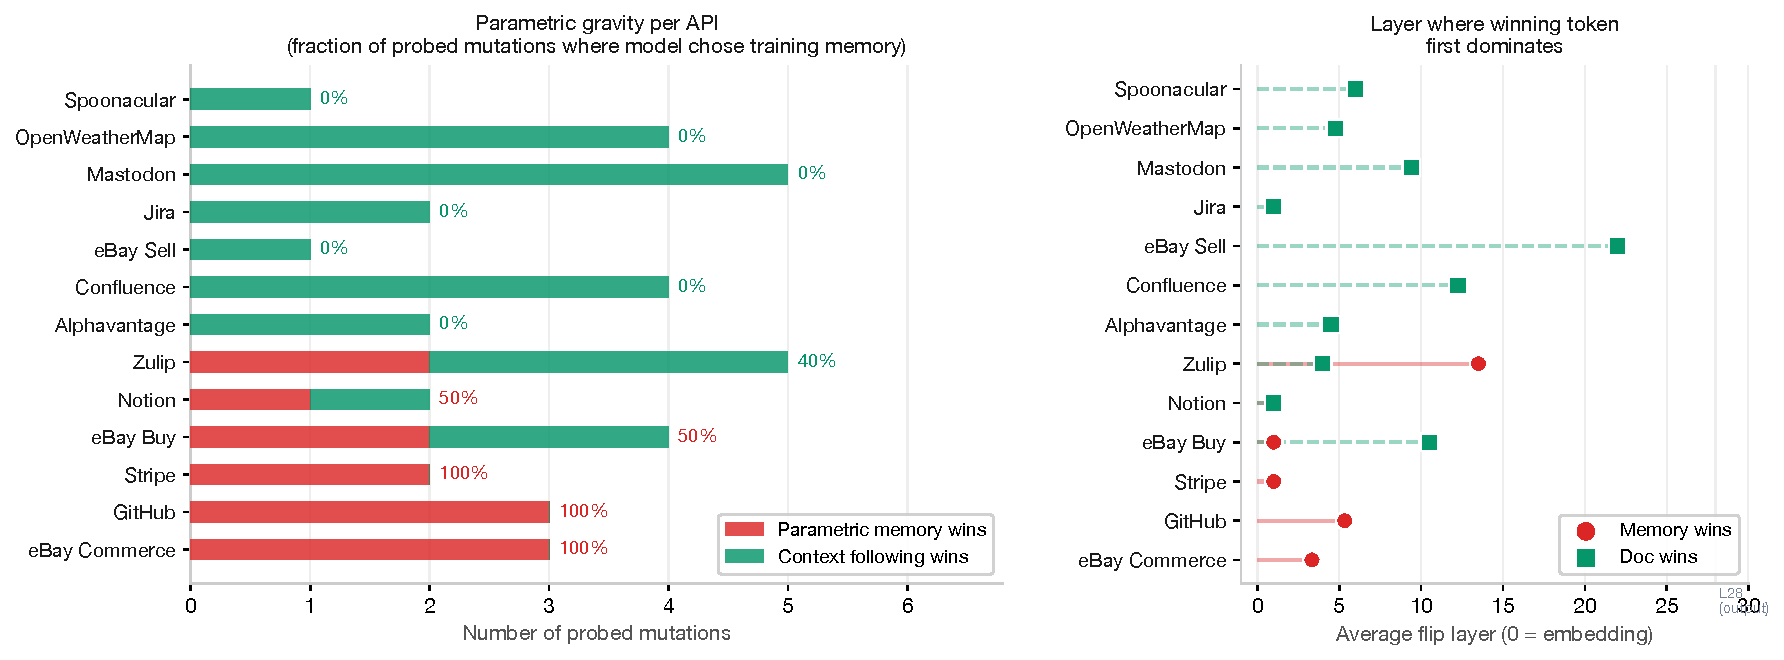
\includegraphics[width=\linewidth]{media/fig_logprobe_summary.pdf}
  \caption{Left: fraction of probed mutations where the model chose the
    training-time parameter name over the in-context mutated name, per API.
    APIs with higher training familiarity (GitHub, Stripe) show 100\% parametric
    memory; less-familiar APIs (Mastodon, Confluence) show full context-following.
    Right: average transformer layer at which the winning token first dominates
    the logit difference. Memory outcomes (red) typically resolve early
    (layers 1--6); context-following outcomes (green) can persist or resolve
    later (eBay Sell: layer 22).}
  \label{fig:logprobe_summary}
\end{figure}

Figure~\ref{fig:logprobe_traces} shows representative layer traces for GitHub (all parametric-memory) and Zulip (mixed). For GitHub parameters such as \texttt{per\_page} and \texttt{state}, $\delta_\ell$ becomes strongly positive within the first few layers and remains so --- the training-time attractor dominates from early in the forward pass. By contrast, Zulip's \texttt{narrow} and \texttt{num\_before} parameters show persistently negative $\delta_\ell$: the model follows the mutated documentation. The Zulip \texttt{anchor} parameter is notable: $\delta_\ell$ stays negative until layer 26, where the parametric attractor abruptly asserts itself --- a late-layer override consistent with a mid-network fact recall mechanism~\citep{meng2022rome}.

\begin{figure}[htbp]
  \centering
  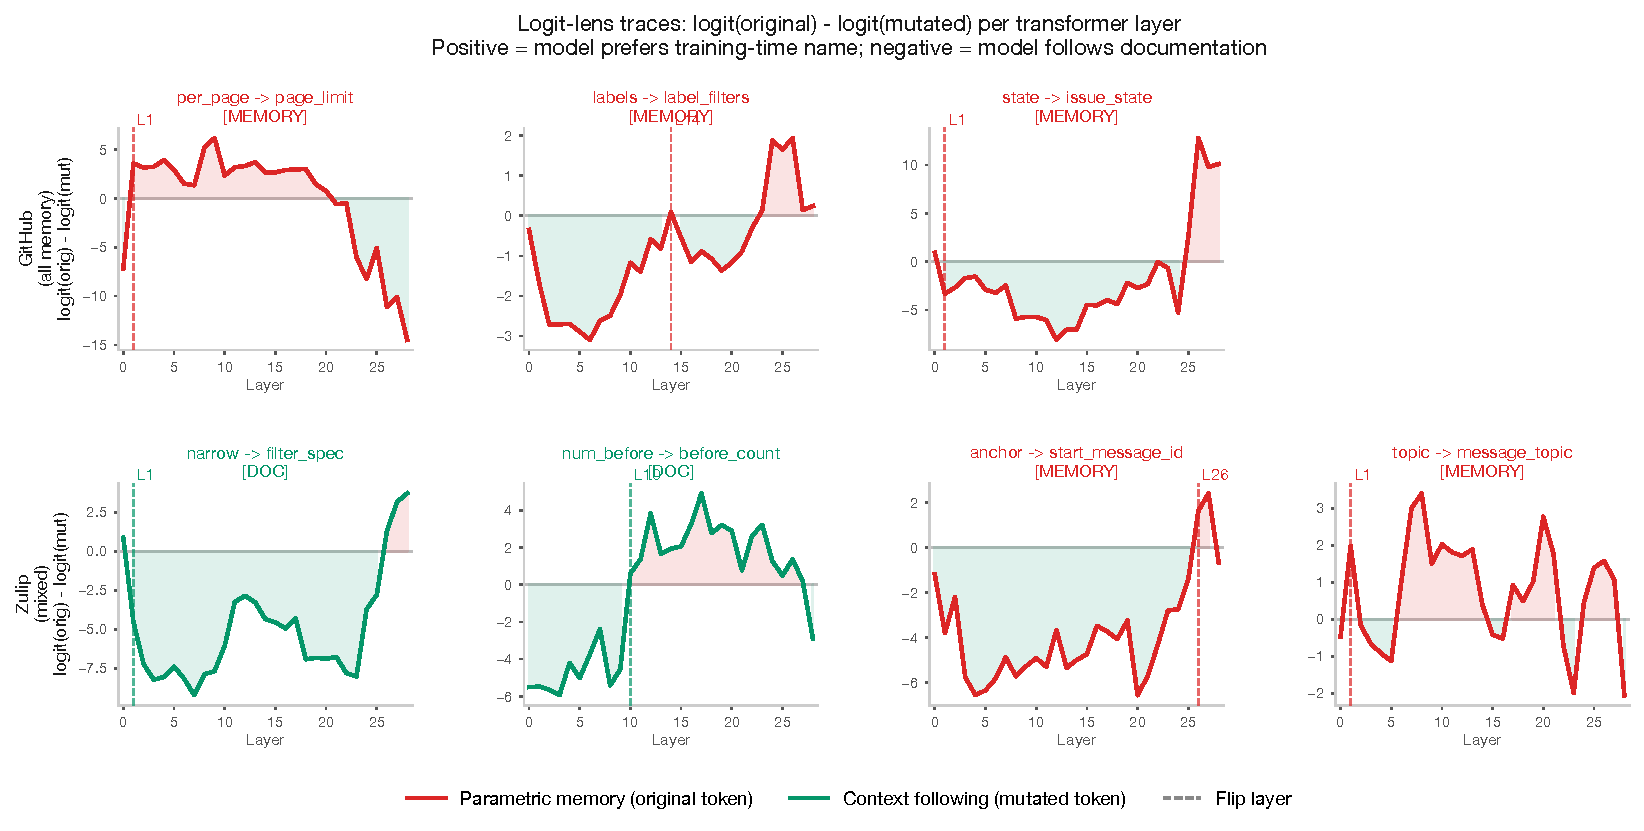
\includegraphics[width=\linewidth]{media/fig_logprobe_traces.pdf}
  \caption{Logit-lens traces for selected GitHub (top row, all memory) and
    Zulip (bottom row, mixed) parameters. Each panel plots
    $\delta_\ell = \text{logit}(\text{original}) - \text{logit}(\text{mutated})$
    across all 29 transformer layers. Positive values (red shading) indicate
    parametric gravity; negative (green shading) indicate context-following.
    The dashed vertical line marks the flip layer. GitHub parameters resolve
    early (L1 for \texttt{per\_page}, \texttt{state}; L14 for \texttt{labels});
    Zulip \texttt{anchor} shows a characteristic late-layer flip at L26.}
  \label{fig:logprobe_traces}
\end{figure}

The average flip layer differs systematically between outcomes: memory-outcome mutations resolve at layers 1--6 on average, while context-following mutations sometimes persist to layer 22 or beyond. This is consistent with parametric gravity being an early-to-mid network phenomenon that, when active, preempts later context integration. APIs without strong attractors reach context-following outcomes gradually throughout the network rather than through a sharp transition.

Mechanistic interpretation of these results --- including their connection to feed-forward fact recall mechanisms and implications for synthesis model choice --- is provided in Section~\ref{sec:discussion-gravity}.
